\documentclass[10pt]{beamer}
\usepackage[utf8]{inputenc}
\usepackage{graphicx}
\usepackage{mathtools}
\usetheme{CambridgeUS}
\usecolortheme{dolphin}
\usepackage{listings}

% Set up hyperref once and configure colors
\usepackage{hyperref}
\hypersetup{
    colorlinks=true,
    linkcolor=blue,
    linktocpage=true
}

% Custom colors
\definecolor{myNewColorA}{RGB}{118,193,188}
\definecolor{myNewColorB}{RGB}{106,172,150}
\definecolor{myNewColorC}{RGB}{94,150,218}
\setbeamercolor*{palette primary}{bg=myNewColorC}
\setbeamercolor*{palette secondary}{bg=myNewColorB, fg=white}
\setbeamercolor*{palette tertiary}{bg=myNewColorA, fg=white}
\setbeamercolor*{titlelike}{fg=myNewColorA}
\setbeamercolor*{title}{bg=myNewColorA, fg=white}
\setbeamercolor*{item}{fg=myNewColorA}
\setbeamercolor*{caption name}{fg=myNewColorA}
\usefonttheme{professionalfonts}

\titlegraphic{
\includegraphics[height=1.5cm]{../CommonFigures/Universidad_Panamericana-logo.jpg}}

\setbeamerfont{title}{size=\large}
\setbeamerfont{subtitle}{size=\small}
\setbeamerfont{author}{size=\small}
\setbeamerfont{date}{size=\small}
\setbeamerfont{institute}{size=\small}
\title[Universidad Panamericana]{}
\subtitle{FreeRTOS Architecture Part 1}
\author[]{Name}
\institute[ltonix@up.edu.mx]{Universidad Panamericana}
\date[Presentation \today]{Presentation \today}

\AtBeginSection[]{
  \begin{frame}
  \vfill
  \centering
  \begin{beamercolorbox}[sep=8pt,center,shadow=true,rounded=true]{title}
    \usebeamerfont{title}\insertsectionhead\par%
  \end{beamercolorbox}
  \vfill
  \end{frame}
}

\setbeamercolor{block title}{bg=myNewColorA, fg=black} % Background and foreground colors for the block title
\setbeamercolor{block body}{bg=myNewColorC, fg=black} % Background and foreground colors for the block body

% Setup listings
\lstset{
  basicstyle=\ttfamily\small,
  keywordstyle=\color{blue},
  commentstyle=\color{green},
  stringstyle=\color{red},
  backgroundcolor=\color{gray!10},
  frame=single,
  language=C++,
  breaklines=true,
  showspaces=false,
  showstringspaces=false
}


\begin{document}

\frame{\titlepage}
\begin{frame}
\frametitle{Contents}
\tableofcontents
\end{frame}

\section{Memory Managment}

\subsection{Memory Hierarchy}
\begin{frame}{Memory Hierarchy: A Light-Hearted Tour}
  \begin{itemize}
    \item \textbf{Registers:} The speed-demons of memory. Too fast to care, but you really should!
    \item \textbf{Cache:} The backseat driver of computing. It makes decisions you didn't ask for, often with surprising results.
    \begin{alertblock}{Friendly Reminder}
      Regularly clearing your cache: not just good practice, it's like digital detox for your devices!
    \end{alertblock}
    \item \textbf{RAM (Random Access Memory):} The workaholic of memory. When it runs out, things go south quickly—plan wisely!
    \item \textbf{Storage:} The elephant's graveyard. Where all your code and files go to rest. Yes, your code lives somewhere physical!
  \end{itemize}
\end{frame}

\begin{frame}{Memory Hierarchy}
  \begin{figure}[h]
    \centering
    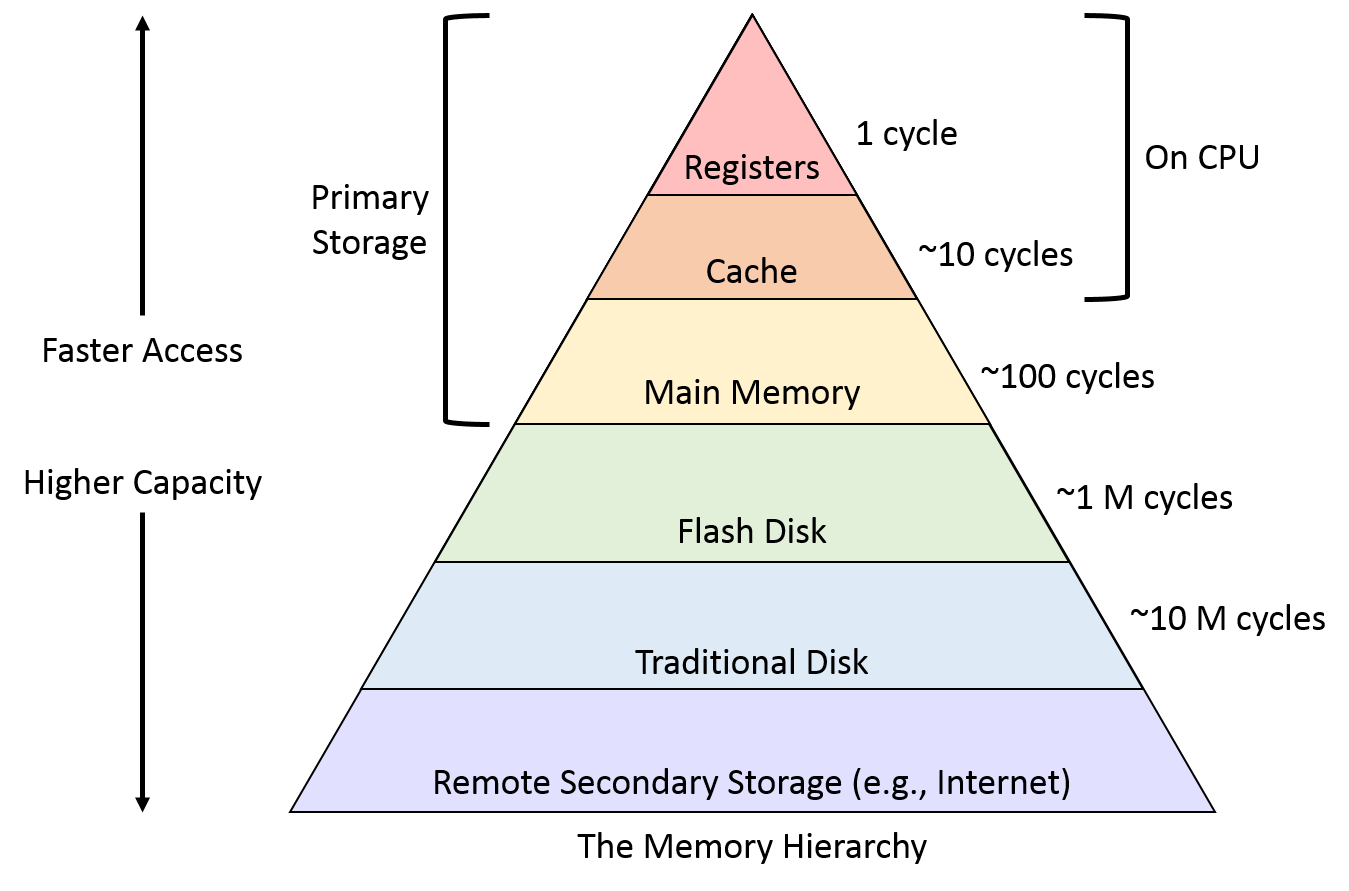
\includegraphics[width=1.0\textwidth]{figures/MemoryHerarchy.png}
    \label{fig:MemoryHerarchy}
  \end{figure}
\end{frame}

\begin{frame}{How does many values has singles variable?}
  \begin{itemize}
    \item One?
    \item Two?
  \end{itemize}
\end{frame}\begin{frame}{How does many values has singles variable?}
  \begin{itemize}
    \item One?
    \item Two?
  \end{itemize}
\end{frame}

\begin{frame}{A variable has two values}
  \begin{itemize}
    \item One : Its current value 
    \item Two : Its current addres
  \end{itemize}
\end{frame}

\subsection{Copy}
\begin{frame}[fragile]{Passing by Copy}
  \begin{itemize}
    \item When parameters are passed by copy, a new instance of the argument is created.
    \item Modifications within the function do not affect the original variable.
    \item Best used when you need to ensure the original data remains unchanged.
\end{itemize}

\begin{lstlisting}
  void incrementByCopy(int x) {
      x = x + 1;
      cout << "Inside function: " << x << endl;
  }
  
  int main() {
      int a = 5;
      incrementByCopy(a);
      cout << "Outside function: " << a << endl;
  }
  \end{lstlisting}

\end{frame}

\subsection{Reference}

\begin{frame}[fragile]{Passing by Reference}
  \begin{itemize}
    \item Passing by reference sends a reference to the original variable.
    \item Any changes inside the function affect the original variable.
    \item More efficient for large data structures but must be used carefully.
  \end{itemize}
  
  \begin{lstlisting}
  void incrementByReference(int& x) {
      x = x + 1;
      cout << "Inside function: " << x << endl;
  }
  
  int main() {
      int a = 5;
      incrementByReference(a);
      cout << "Outside function: " << a << endl;
  }
  \end{lstlisting}
\end{frame}

\begin{frame}
  \begin{figure}[h]
    \centering
    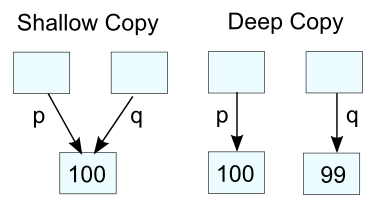
\includegraphics[width=1.0\textwidth]{figures/deep_vs_shallow_copy.png}
    \label{fig:MemoryHerarchy}
  \end{figure}
\end{frame}

\section{Stack and Heap memory}
\begin{frame}{Stack Memory}
  \begin{itemize}
    \item \textbf{Definition:} Stack memory is a region of memory where data is added or removed in a last-in-first-out (LIFO) manner.
    \item \textbf{Usage:} Primarily used for static memory allocation, including function call stack (local variables, function parameters).
    \item \textbf{Characteristics:}
      \begin{itemize}
        \item Fixed size, typically allocated at the start of the program.
        \item Automatic management, with variables being pushed \{ onto the stack and popped off \}when no longer needed.
        \item Yes the \{ and \} mean something in the code!!! \href{run:./QuizzSwitchCase.cpp}{\texttt{QuizzSwitchCase.cpp}}
        \item Fast access due to locality of reference and simplicity of allocation mechanism (moving the stack pointer).
      \end{itemize}
    \item \textbf{Limitations:}
      \begin{itemize}
        \item Limited space, which can lead to stack overflow if too many function calls or large arrays are declared.
        \item No resizing, and not suitable for dynamically allocated data.
      \end{itemize}
  \end{itemize}
\end{frame}

\begin{frame}{Heap Memory}
  \begin{itemize}
    \item \textbf{Definition:} Heap memory is a region of memory used for dynamic memory allocation where blocks of memory are allocated and freed in an arbitrary order.
    \item \textbf{Usage:} Utilized for allocating memory at runtime when the amount of memory needed cannot be determined at compile time.
    \item \textbf{Characteristics:}
      \begin{itemize}
        \item Dynamically grows and shrinks based on application needs.
        \item Managed through library routines or operating system functions like malloc() and free() in C.
        \item Flexible, but with higher overhead and slower access compared to stack memory.
      \end{itemize}
    \item \textbf{Limitations:}
      \begin{itemize}
        \item Can lead to memory fragmentation.
        \item User error for bad manual handling. \href{run:./BadLinkedList.cpp}{\texttt{BadLinkedList.cpp}}
      \end{itemize}
  \end{itemize}
\end{frame}

\section{Function Pointers}
\begin{frame}{Function Pointers}
  \begin{itemize}
    \item \textbf{What Are They?} Variables that store the address of a function.
    \item \textbf{Use Cases:}
      \begin{itemize}
        \item Modular software design.
        \item Passing functions as arguments.
      \end{itemize}
    \item \textbf{Syntax Example:}
      \begin{itemize}
        \item \texttt{void (*funPtr)(int) = \&fun;}
      \end{itemize}
  \end{itemize}
\end{frame}

\subsection{Callbacks}
\begin{frame}{Callbacks}
  \begin{itemize}
    \item \textbf{Definition:} Functions passed as arguments to other functions.
    \item \textbf{Purpose:}
      \begin{itemize}
        \item Allow a lower-level software layer to call a function in a higher-level layer.
        \item Used extensively for event-driven programming.
      \end{itemize}
    \item \textbf{Example Use:}
      \begin{itemize}
        \item Asynchronous data processing.
        \item Reacting to user inputs or software events.
      \end{itemize}
  \end{itemize}
\end{frame}

\section{FreeRTOS}
\subsection{Task}
\begin{frame}{Task similar to Function Pointer}
  \begin{itemize}
    \item \textbf{Task as Function Pointer:}
      \begin{itemize}
        \item In FreeRTOS, tasks are defined by function pointers.
        \item Function defines task behavior and is invoked when the task runs.
      \end{itemize}
    \item \textbf{How It Works:}
      \begin{itemize}
        \item \texttt{xTaskCreate(pvTaskCode, "TaskName", STACK\_SIZE, NULL, Priority, NULL);}
      \end{itemize}
    \item \textbf{Advantages:}
      \begin{itemize}
        \item Flexibility in task management.
        \item Easy integration of different functionalities.
      \end{itemize}
  \end{itemize}
\end{frame}

\subsection{Scheduler}

\begin{frame}{Task States in FreeRTOS}

  \begin{figure}[h]
    \centering
    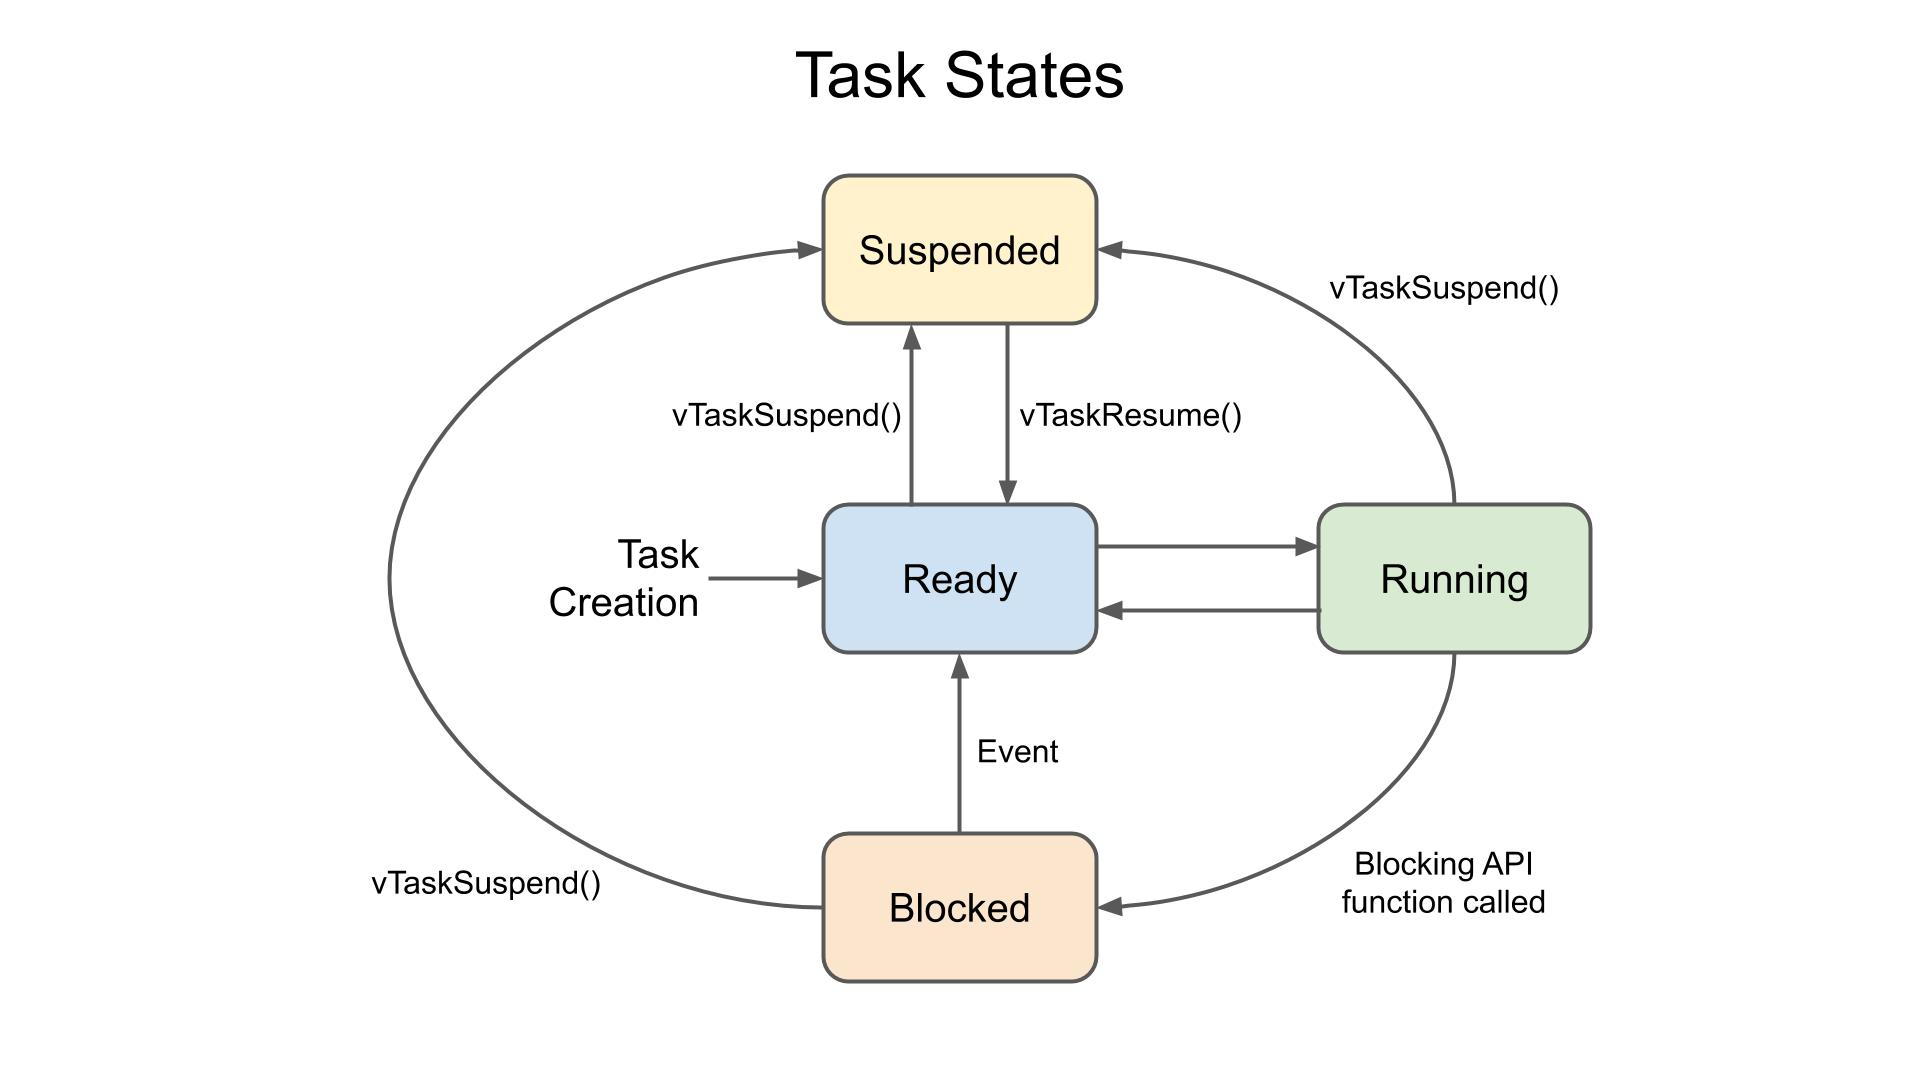
\includegraphics[width=1.0\textwidth]{figures/FreeRTOScheduling.jpeg}
    \label{fig:FreeRTOScheduling}
  \end{figure}
\end{frame}


\begin{frame}{Task States in FreeRTOS}
  \frametitle{Understanding Task States}
  \begin{itemize}
    \item \textbf{Task Creation}: A new task starts in the \textit{Ready} state, waiting to be scheduled to run.
    \item \textbf{Ready}: Tasks in this state are ready to run but are currently not being executed by the CPU.
    \item \textbf{Running}: The state of the currently executing task. Only one task can be in this state at a time on single-core systems.
    \item \textbf{Blocked}: A task enters this state if it cannot continue because it is waiting for an event or resource. It will remain blocked until the event occurs or the resource becomes available.
    \item \textbf{Suspended}: Tasks in this state are intentionally suspended by the application, possibly to conserve power or CPU time. They are not schedulable until they are explicitly resumed.
    \item \textbf{Transitions}:
  \end{itemize}
 
\end{frame}

\begin{frame}{Task States in FreeRTOS}
  \begin{itemize}
    \item \textit{vTaskSuspend()} moves a task to \textit{Suspended}.
    \item \textit{vTaskResume()} moves a task from \textit{Suspended} back to \textit{Ready}.
    \item An event or the availability of a resource moves a task from \textit{Blocked} to \textit{Ready}.
    \item Tasks switch from \textit{Ready} to \textit{Running} based on scheduler decisions and priority.
  \end{itemize}
  \begin{block}{Note}
    Only the scheduler can move tasks into the \textit{Running} state or handle transitions when a blocking API function is called.
  \end{block}
\end{frame}

\subsection{Systick}
\begin{frame}{SysTick Timer}
  \frametitle{SysTick Timer in FreeRTOS}
  \begin{itemize}
    \item \textbf{Purpose:} The SysTick timer generates interrupt requests at a selectable interval and is often used to increment the system tick count in RTOS.
    \item \textbf{Function:} Essential for task scheduling, timekeeping, and implementing time delays.
    \item \textbf{System Tick:} Typically configured to tick once per millisecond, which serves as the heartbeat for task switches and timing operations.
  \end{itemize}
  \end{frame}

\subsection{VtaskDelay}
\begin{frame}{Impact of vTaskDelay on Scheduler States}
  \frametitle{Task Management and Scheduler States}
  \begin{itemize}
    \item \textbf{vTaskDelay:} Delays the execution of the current task, allowing other tasks to run.
    \item \textbf{Scheduler States:}
      \begin{itemize}
        \item \textbf{Running:} The currently executing task.
        \item \textbf{Ready:} Tasks that are ready to run when given CPU time.
        \item \textbf{Blocked:} `vTaskDelay` moves the task to the Blocked state until the delay time expires.
        \item \textbf{Suspended:} Tasks that have been explicitly suspended, not affected by `vTaskDelay`.
      \end{itemize}
    \item \textbf{Task Switching:} `vTaskDelay` can trigger a context switch if a higher priority task is ready to run.
  \end{itemize}
  \end{frame}

\begin{frame}[fragile]{Code Example: Using vTaskDelay}
    \frametitle{Practical Usage of vTaskDelay}
    \begin{lstlisting}[language=C]
    #include "FreeRTOS.h"
    #include "task.h"
    
    void vTaskCode(void *pvParameters)
    {
        for (;;)
        {
            // Perform task operation
            printf("Task is running.\n");
            // Delay the task for 100 ticks
            vTaskDelay(100);
            printf("Task resumes after delay.\n");
        }
    }
    \end{lstlisting}
\end{frame}

\end{document}